\documentclass[aspectratio=169,10pt]{beamer}
\usetheme{Boadilla}
\usecolortheme{default}
\definecolor{ink}{HTML}{1F2937}
\definecolor{accent}{HTML}{2A78D6}
\definecolor{accent2}{HTML}{EB6834}
\definecolor{soft}{HTML}{EEF3FA}
\setbeamercolor{structure}{fg=accent}
\setbeamercolor{palette primary}{bg=accent,fg=white}
\setbeamercolor{palette secondary}{bg=accent!80!black,fg=white}
\setbeamercolor{palette tertiary}{bg=accent!60!black,fg=white}
\setbeamercolor{title}{fg=ink}
\setbeamercolor{frametitle}{bg=accent,fg=white}
\setbeamercolor{block title}{bg=accent,fg=white}
\setbeamercolor{block body}{bg=soft}
\setbeamercolor{alerted text}{fg=accent2}
\setbeamerfont{frametitle}{series=\bfseries}
\setbeamertemplate{navigation symbols}{}
\setbeamertemplate{itemize items}[circle]
\setbeamertemplate{sections/subsections in toc}[ball]
\setbeamertemplate{caption}{\raggedright\insertcaption\par}
\usepackage{booktabs,amsmath,amssymb,graphicx,tikz}
\usetikzlibrary{arrows.meta,positioning,shapes.geometric}
\setbeamertemplate{itemize/enumerate body begin}{\setlength{\itemsep}{3pt}}
\newcommand{\hi}[1]{\textcolor{accent2}{\textbf{#1}}}
\newcommand{\pyes}{p}

\title[Learned deferral for sanctions ER]{Learned deferral for sanctions entity resolution\\\large Classical matchers, LLMs and human review}
\author{Harsh Chauhan}
\institute[IIT Dharwad]{Pattern Recognition and Machine Learning, course project\\Indian Institute of Technology Dharwad}
\date{November 2026}

\begin{document}

\begin{frame}[plain]
\titlepage
\end{frame}

\begin{frame}{Outline}
\tableofcontents
\end{frame}

% ============================================================
\section{Motivation}

\begin{frame}{Entity resolution in sanctions screening}
\begin{itemize}
\item Entity resolution asks whether two records from different sources describe the same real-world person, company or vessel.
\item Banks, payment companies, exchanges and investigative journalists screen customer and counterparty names against sanctions and watch lists every day. OpenSanctions alone merges records from 293 sources into about a million entities.
\item Both mistakes are costly. A missed match lets a sanctioned entity through, which is a legal and reputational problem. A false match blocks a legitimate customer and sends the case to an analyst.
\item Analyst review is the expensive part. The practical question is not only ``is this a match'' but ``which pairs deserve a human look''.
\end{itemize}
\end{frame}

\begin{frame}{Why it is hard}
\begin{columns}[T]
\begin{column}{0.5\textwidth}
\begin{itemize}
\item The same person appears under different transliterations, name orders and scripts, and often under aliases.
\item Sources record different subsets of fields. One list gives a birth date and a position, another a birth place and an identifier, a third only a name.
\item Different people share names. Namesakes can only be separated by dates, places and identifiers, and those are often missing.
\item Data-entry errors are common, so a conflicting date or identifier is not proof of a different entity.
\end{itemize}
\end{column}
\begin{column}{0.48\textwidth}
\begin{block}{Record A (sanctions list 1)}
\scriptsize\ttfamily
type: Person\\
name: Vitaliy Anatolyevich Markelov\\
other names: MARKELOV, Vitaliy; Markelov Vitaly Anatolievich\\
birth date: 1963-08-05 \quad nationality: ru\\
position: Deputy Chairman, Gazprom
\end{block}
\begin{block}{Record B (sanctions list 2)}
\scriptsize\ttfamily
type: Person\\
name: Witalij Anatoljewicz Markielow\\
birth date: 1963-08-05 \quad citizenship: ru\\
birth place: Mordovia \quad wikidata: Q114246932
\end{block}
\small The analysts labelled this pair \hi{same entity}.
\end{column}
\end{columns}
\end{frame}

\begin{frame}{The OpenSanctions Pairs benchmark}
\begin{itemize}
\item OpenSanctions released the first large public benchmark for this task in 2026. It has 755{,}540 record pairs judged by their analysts, drawn from over a million entities, 293 sources and 45 jurisdictions.
\item Their paper reports 91.3 F1 for the production scorer, a small regression over a few rule features, and 94 to 99 F1 for LLMs from Llama 8B up to GPT-4o.
\item They name uncertainty-aware review as the open problem. Nobody has studied which pairs should go to a human and what that review buys.
\item Nothing stronger than the small regression scorer has been trained on these 755k labels, although labelled pairs are exactly what supervised record linkage needs.
\end{itemize}
\end{frame}

\begin{frame}{The gap and our three questions}
\begin{itemize}
\item \hi{Question 1.} How good is a supervised classical matcher trained on these labels, and how many labels does it need?
\item \hi{Question 2.} Given a cheap matcher and an expensive expert, which pairs should be handed over, and how much does a fixed review budget buy?
\item \hi{Question 3.} Are LLM errors complementary to matcher errors? If not, an LLM is a poor expert however good it is on average.
\item The tools are from this course. Seven classifiers with cross-validation, probability calibration, and Bayes decision theory with a reject option.
\item In one line, a random forest beats the LLMs, handing 5\% of pairs to a human removes 71\% of the remaining errors, and handing them to an LLM barely helps.
\end{itemize}
\end{frame}

% ============================================================
\section{Data and features}

\begin{frame}{Data}
\begin{itemize}
\item Source file \texttt{pairs-20251209.json.gz}, public under CC BY-NC. Each record has a schema (Person, Company, Vessel and so on), names and aliases, birth date, nationality, identifiers and addresses, plus the analyst label.
\item Provenance fields that could leak the label (\texttt{datasets}, \texttt{referents}, \texttt{first\_seen}, \texttt{target}) are dropped first.
\item 280{,}487 lines (37\%) are auto-generated relational stubs such as Occupancy or Ownership records. Both sides are byte-identical and the label is always positive. A first run that included them reported a meaningless 99.4 F1. Reading the LLM's ``mistakes'' (Occupancy vs Occupancy) exposed it. Only the ten entity schemas are kept.
\item After de-duplication there are 264k positive and 171k negative unique pairs. We sample 39k positive and 21k negative with a fixed seed and split them 36k, 6k, 18k for train, validation and test.
\end{itemize}
\end{frame}

\begin{frame}{Features}
\begin{itemize}
\item A classifier cannot read two JSON records, so each pair is turned into 29 numbers that describe how the two records relate.
\item Names. Best Jaro-Winkler, token-set ratio, token Jaccard and Levenshtein ratio over all name pairs, exact normalised-name match, first and last name overlap, and a flag for different scripts.
\item Type and dates. Agreement of entity type, whether both sides have a date, whether the full dates or the years match, the year gap, and a missing-date flag.
\item Geography, gender and identifiers. Nationality and country overlap and conflict, gender mismatch, and whether identifiers are present on both sides, match, or conflict.
\item Other fields. Address, topic, position and birthplace overlap.
\item Five more features that count names and properties per record were computed but dropped. They leak how often an entity appears in the dataset, which correlates with the label.
\end{itemize}
\end{frame}

% ============================================================
\section{Methods, theory and implementation}

\begin{frame}{The pipeline}
\centering
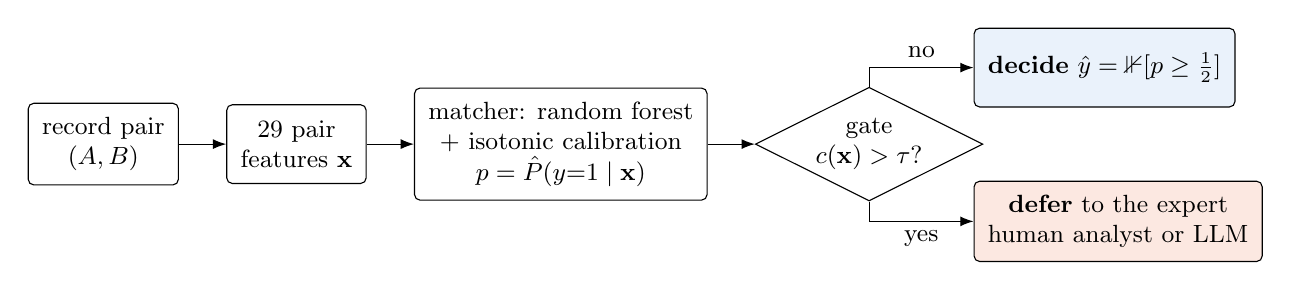
\begin{tikzpicture}[font=\small,>=Latex,node distance=6mm,
 box/.style={draw,rounded corners=2pt,align=center,inner sep=5pt,minimum height=10mm,fill=white},
 dec/.style={draw,diamond,aspect=2.0,align=center,inner sep=1pt,fill=white}]
\node[box] (rec) {record pair\\$(A,B)$};
\node[box,right=of rec] (feat) {29 pair\\features $\mathbf{x}$};
\node[box,right=of feat] (rf) {matcher: random forest\\+ isotonic calibration\\$\pyes=\hat P(y{=}1\mid\mathbf{x})$};
\node[dec,right=of rf] (gate) {gate\\$c(\mathbf{x})>\tau$?};
\node[box,above right=1mm and 6mm of gate,fill=accent!10] (acc) {\textbf{decide} $\hat y=\mathbb{1}[\pyes\ge\tfrac12]$};
\node[box,below right=1mm and 6mm of gate,fill=accent2!15] (exp) {\textbf{defer} to the expert\\human analyst or LLM};
\draw[->] (rec)--(feat); \draw[->] (feat)--(rf); \draw[->] (rf)--(gate);
\draw[->] (gate)|- node[pos=0.75,above]{no} (acc);
\draw[->] (gate)|- node[pos=0.75,below]{yes} (exp);
\end{tikzpicture}
\begin{itemize}
\item The matcher turns the features into a calibrated posterior $p$ for ``same entity''.
\item The gate turns $p$ (and optionally $\mathbf{x}$) into a score $c(\mathbf{x})$ and defers the pairs above a threshold $\tau$ set by the review budget.
\item The expert answers the deferred pairs. Everything upstream is shared, so the human and the LLMs are compared on exactly the same pairs.
\end{itemize}
\end{frame}

\begin{frame}{The seven classifiers}
\footnotesize
\begin{tabular}{@{}p{0.2\textwidth}p{0.47\textwidth}p{0.27\textwidth}@{}}
\toprule
method & idea & setting used\\
\midrule
logistic regression & linear decision boundary on standardised features, probability through the sigmoid & L2 penalty, $C=1$, balanced class weights\\
SVM with RBF kernel & maximum-margin boundary in the kernel feature space, non-linear through the Gaussian kernel & $C=3$, $\gamma$ = scale, Platt scaling for probabilities\\
$k$-nearest neighbours & vote of the nearest training pairs in standardised feature space, weighted by inverse distance & $k=25$\\
decision tree & greedy axis-aligned splits that reduce Gini impurity & depth 8, at least 20 pairs per leaf\\
random forest & bagging of deep trees with random feature subsets, vote fraction as score & 400 trees, min leaf 2, balanced subsample weights\\
AdaBoost & re-weights the misclassified pairs and adds a shallow tree each round & 300 depth-2 trees, learning rate 0.5\\
gradient boosting & fits each new tree to the gradient of the log loss & 400 iterations, learning rate 0.06, 31 leaves\\
\bottomrule
\end{tabular}
\vspace{2mm}
\begin{itemize}
\item All seven see the same 29 features and the same 36k training pairs. Class weights handle the 65 to 35 imbalance.
\end{itemize}
\end{frame}

\begin{frame}{Model selection and evaluation protocol}
\begin{itemize}
\item Model selection uses 5-fold stratified cross-validation on the 36k training pairs. The out-of-fold predictions give the CV F1 and AUC of every classifier, and the forest wins on both.
\item The operating threshold is chosen on the 6k validation split to maximise F1, then frozen. For the forest it is 0.5 anyway.
\item The 18k test pairs are scored once per classifier. We report F1, precision, recall, accuracy, ROC AUC and the Brier score.
\item Leakage controls. Provenance fields removed, relational stubs removed, an entity-overlap check between the splits, and an ablation of the count features.
\item Uncertainty. All seeds are fixed for the sample, the split and every model, and the full-population check carries a 200-sample bootstrap confidence interval.
\end{itemize}
\end{frame}

\begin{frame}{Probability calibration}
\begin{itemize}
\item The forest's vote fraction $s$ ranks pairs very well (AUC 0.997), but it is a score, not a probability. The reject rule thresholds on $\min(p,1-p)$, so it needs a probability.
\item Isotonic regression fits a monotone non-decreasing map $g$ to the validation split with the pool-adjacent-violators algorithm, and the calibrated posterior is $p=g(s)$:
\[
g=\arg\min_{g\ \text{non-decreasing}}\ \sum_{i\in\text{val}}\bigl(y_i-g(s_i)\bigr)^2 .
\]
\item It is fitted on the 6k validation pairs, never on test, and it only reshapes the scale, so the ranking and the AUC are unchanged.
\item On test the Brier score moves from 0.0140 to 0.0137, F1 from 98.68 to 98.72, and the reliability curve lies on the diagonal. The confidence score $\min(p,1-p)$ is now meaningful.
\end{itemize}
\end{frame}

\begin{frame}{Bayes decision theory with a reject option}
\begin{itemize}
\item Three actions are available for a pair with posterior $p$. Say match, with expected loss $(1-p)\,c_{\mathrm{FP}}$. Say different, with expected loss $p\,c_{\mathrm{FN}}$. Defer to the expert, at a fixed cost $c_d$.
\item The Bayes rule picks the smallest expected loss, so the pair is deferred exactly when
\[
\frac{c_d}{c_{\mathrm{FN}}}\;<\;p\;<\;1-\frac{c_d}{c_{\mathrm{FP}}}\,,
\qquad\text{and with equal costs}\qquad \min(p,\,1-p)>\lambda
\]
which is Chow's reject rule (1970, Bishop 1.5.3). Asymmetric costs shift the region towards the cheap mistake.
\item A review team of fixed size needs the budget form. Rank pairs by $\min(p,1-p)$ and defer the top fraction $b$, which traces the whole curve of F1 against budget.
\item Two bounds bracket every gate. The random gate defers $b$ pairs at random, the oracle gate defers exactly the wrong pairs.
\end{itemize}
\end{frame}

\begin{frame}{Learning to defer, the learned gates}
\begin{itemize}
\item The confidence gate ignores the features. A learned gate can use them. The error gate estimates $\hat P(\text{matcher wrong}\mid\mathbf{x},p,s)$. The gain gate estimates $\hat P(\text{expert right and matcher wrong}\mid\mathbf{x},p,s)$, which is the quantity that should drive deferral to an imperfect expert.
\item Both are ordinary classifiers, logistic regression and gradient boosting with balanced class weights, trained on 12k training pairs that also have LLM answers. These pairs are disjoint from the calibration and test splits.
\item Each gate score ranks the test pairs, so every gate is compared at the same budgets, and the AUC of the score against the matcher's actual errors measures gate quality directly.
\item The learned gates have more information than the confidence gate. Whether they use it is an empirical question, answered in the results.
\end{itemize}
\end{frame}

\begin{frame}{The LLM as a matcher and as an expert}
\begin{itemize}
\item Models. Qwen2.5-7B-Instruct in bf16, Qwen2.5-14B-Instruct in 4-bit AWQ, and a four-shot variant of the 7B model, all served with vLLM at temperature 0.
\item Prompt. ``You are an expert analyst doing entity resolution on sanctions and watchlist data. Decide whether the two records below refer to the same real-world entity. Names may be transliterated differently, abbreviated or only partially listed. Minor inconsistencies in dates or identifiers are often data-entry errors. Different people can share a name, so use dates, places and identifiers to disambiguate. Record A. Record B. Answer with exactly one word, yes or no.''
\item The records are rendered as labelled lines, 417 prompt tokens on average. The model answers with one word and $P(\text{yes})$ is read from the first-token log probabilities.
\item As a matcher its answer is scored like any classifier. As an expert its answer replaces the matcher's on the deferred pairs. A 600-pair validation check (95.9 F1) preceded the 30k-pair runs (95.8).
\end{itemize}
\end{frame}

\begin{frame}{Implementation}
\begin{itemize}
\item Python with scikit-learn for every classical model, rapidfuzz for string similarity and vLLM for the LLMs. About 2{,}000 lines in 13 scripts, one per stage, plus an executed notebook that runs every stage and keeps its outputs.
\item Runtimes. Sampling, splitting and featurising 60k pairs takes about 3 minutes. All seven classifiers with cross-validation take about a minute on CPU (the SVM 13 s, the forest 7 s). Scoring 30k pairs with the LLMs took 376 s, 850 s and 403 s on an H100 MIG slice. Gates and deferral curves take seconds.
\item Hardware. The ml.cern.ch JupyterLab service. Everything except the LLM runs is CPU only and reproduces in minutes.
\item Reproducibility. Fixed seeds, the saved split, every number in one results file, every figure regenerated by one script, and a demo script that retrains the matcher and recomputes the curves live.
\end{itemize}
\end{frame}

% ============================================================
\section{Results}

\begin{frame}{Matcher results}
\begin{columns}[T]
\begin{column}{0.47\textwidth}
\footnotesize
\begin{tabular}{@{}lccc@{}}
\toprule
classifier & CV F1 & test F1 & AUC\\
\midrule
logistic regression & 96.5 & 97.1 & 0.989\\
decision tree & 98.1 & 98.1 & 0.992\\
AdaBoost & 98.0 & 98.0 & 0.995\\
SVM (RBF) & 98.5 & 98.5 & 0.995\\
kNN & 98.5 & 98.6 & 0.995\\
gradient boosting & 98.7 & 98.6 & 0.997\\
\textbf{random forest} & \textbf{98.7} & \hi{98.7} & \textbf{0.997}\\
\midrule
Qwen2.5-7B zero-shot & & 95.8 & \\
Qwen2.5-14B zero-shot & & 96.6 & \\
best single rule & & 94.6 & \\
production scorer & & 91.3 & \\
\bottomrule
\end{tabular}
\end{column}
\begin{column}{0.51\textwidth}
\begin{itemize}
\item Cross-validation and test agree within 0.1 for every model, so nothing is tuned to the test split.
\item The best single rule is a token-set ratio above 0.99. The production scorer value is the one reported in the benchmark paper.
\item The same forest applied to all \hi{375{,}842 other pairs} of the benchmark gives 98.5 F1 (95\% CI 98.4 to 98.5) with the same AUC, so the sample was not lucky.
\end{itemize}
\end{column}
\end{columns}
\end{frame}

\begin{frame}{How many labels does the matcher need}
\begin{columns}[T]
\begin{column}{0.5\textwidth}
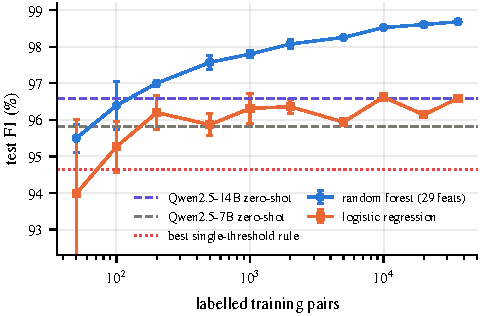
\includegraphics[width=\textwidth]{fig_learning_curve.pdf}
\end{column}
\begin{column}{0.48\textwidth}
\begin{itemize}
\item With 100 labelled pairs the forest already matches the 7B LLM (96.4 vs 95.8). With 1{,}000 it reaches 97.8, with 10k 98.5, and it saturates near 98.7.
\item Logistic regression stays between 96 and 97 at every size, so the gain comes from interactions between features, not from more data.
\item A few hundred analyst labels buy more than a 7B model.
\end{itemize}
\end{column}
\end{columns}
\end{frame}

\begin{frame}{Deferring to a human analyst}
\begin{columns}[T]
\begin{column}{0.52\textwidth}
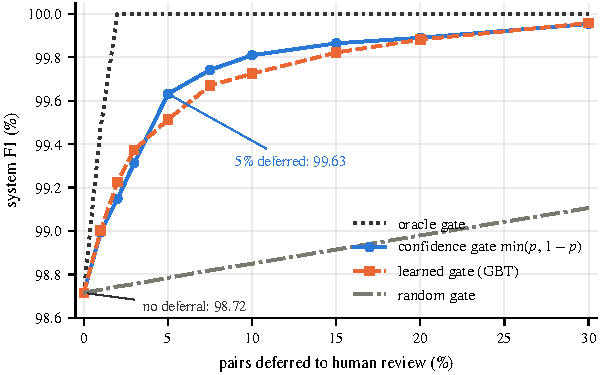
\includegraphics[width=\textwidth]{fig_deferral_human.pdf}
\end{column}
\begin{column}{0.46\textwidth}
\begin{itemize}
\item Reviewing the 5\% least confident pairs removes \hi{71\% of the remaining errors}. F1 rises from 98.7 to 99.6 and the error count falls from 304 to 87.
\item Reviewing 10\% removes 85\%. A random 5\% removes only 5\%.
\item An oracle gate would need just 2\%, so the gap between confidence and oracle is the room left for a better gate.
\item The learned gates do not beat plain confidence at any budget. The forest's calibrated uncertainty is already the signal.
\end{itemize}
\end{column}
\end{columns}
\end{frame}

\begin{frame}{The reviewer need not be perfect and the costs need not be equal}
\begin{columns}[T]
\begin{column}{0.5\textwidth}
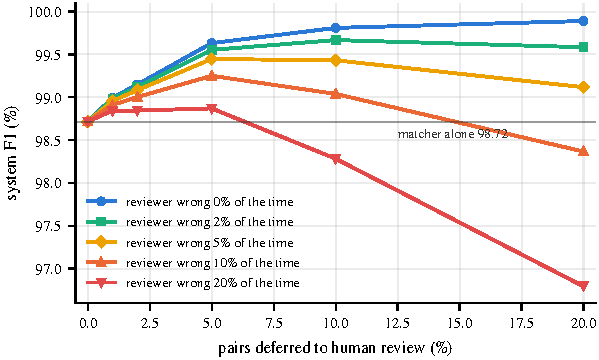
\includegraphics[width=0.93\textwidth]{fig_noisy_human.pdf}
\begin{itemize}
\item \footnotesize The matcher is wrong on 24\% of the pairs it defers at a 5\% budget, so a reviewer who is wrong 10\% of the time still lifts F1 to 99.25, and one wrong 20\% of the time still helps. Deferral pays as long as the reviewer beats 24\% on those pairs.
\end{itemize}
\end{column}
\begin{column}{0.5\textwidth}
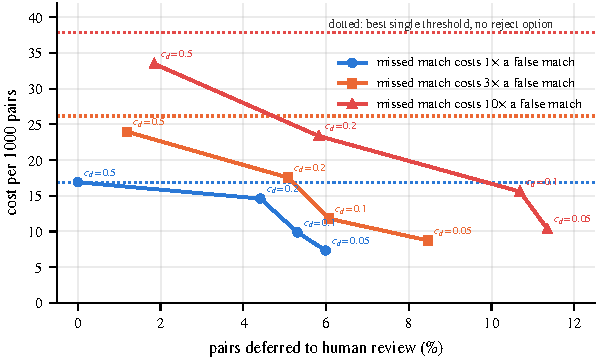
\includegraphics[width=0.93\textwidth]{fig_cost.pdf}
\begin{itemize}
\item \footnotesize With a missed match costing 10 times a false match, the Bayes reject region becomes $0.01<p<0.9$, 10.7\% of pairs are deferred, misses drop from 24 to 3 and the cost per 1000 pairs falls from 37.9 to 15.6.
\end{itemize}
\end{column}
\end{columns}
\end{frame}

\begin{frame}{Deferring to an LLM}
\begin{columns}[T]
\begin{column}{0.52\textwidth}
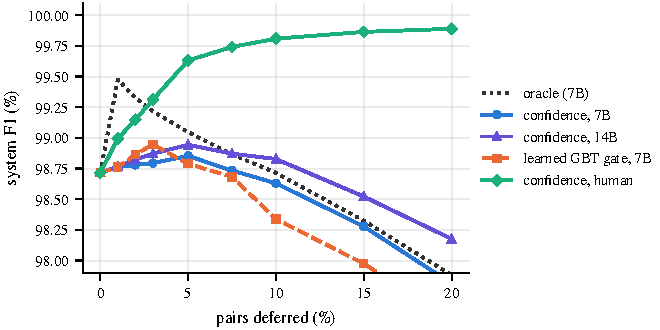
\includegraphics[width=\textwidth]{fig_deferral_zoom.pdf}
\end{column}
\begin{column}{0.46\textwidth}
\small
\begin{itemize}
\item Handing the least confident 5\% to Qwen2.5-7B moves F1 from 98.72 to 98.85. The 14B model reaches 98.94. Past 10\% the curves turn down, and at 100\% it is the LLM alone at 95.8.
\item Four-shot prompting makes the LLM worse, 94.5 alone and no gain as an expert.
\item Combining instead of deferring gives the same answer. A tuned weighted average, a logistic stacker and the LLM probability as a 30th forest feature all land at 98.9.
\item At any size or prompt the LLM adds \hi{at most 0.2 F1}, against 0.9 for a human at the same budget.
\end{itemize}
\end{column}
\end{columns}
\end{frame}

\begin{frame}{Why the LLM does not help}
\begin{columns}[T]
\begin{column}{0.5\textwidth}
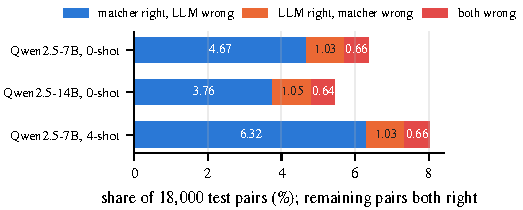
\includegraphics[width=0.9\textwidth]{fig_complementarity.pdf}
\begin{block}{\small Analyst: different. Matcher 1.00, every LLM: yes}
\scriptsize\ttfamily A: Vitaliy Anatolyevich Markelov, 1963-08-05, Mordovia\\B: Vitaliy Anatolyevich Maarkelov, 1963-08-05, Mordovia
\end{block}
\begin{block}{\small Analyst: different. Matcher 0.97, every LLM: yes}
\scriptsize\ttfamily A: Person, [Thai-script name], nationality th, Legislative Assembly\\B: Person, identical name, male, nationality th, same position
\end{block}
\end{column}
\begin{column}{0.48\textwidth}
\small
\begin{itemize}
\item On the 18k test pairs, 93.6\% are right for both systems, 4.7\% only the matcher gets right, 1.0\% only the LLM, and 0.66\% nobody.
\item 89 pairs are wrong for the matcher and all three LLM configurations. They share a name but have no dates or identifiers, and the analysts judged them different. 42\% of them get $p\ge 0.95$ from the forest, so they are confidently wrong rather than uncertain.
\item This information is not in the records, so a bigger model will not recover it. Some are probable label errors. The reject option is the right answer here.
\end{itemize}
\end{column}
\end{columns}
\end{frame}


\begin{frame}{Does a bigger, reasoning model change this}
\centering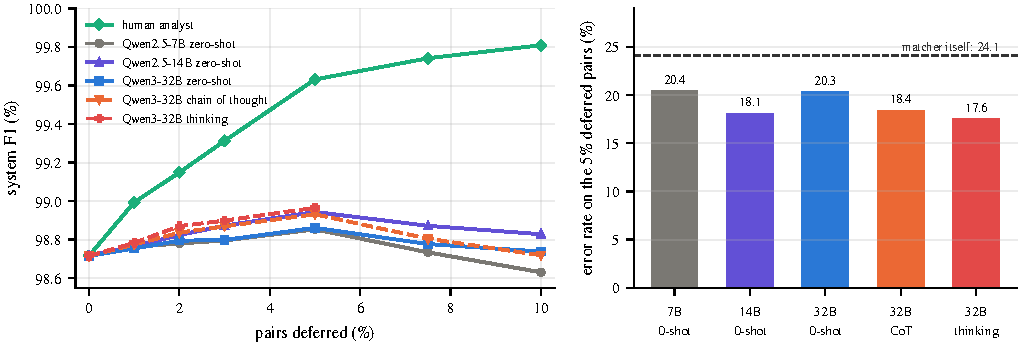
\includegraphics[width=0.8\textwidth]{fig_experts.pdf}
\vspace{-1mm}
\footnotesize
\begin{itemize}
\item Qwen3-32B-AWQ, four times the parameters, run zero-shot on all 30k pairs, with a short chain of thought on the 10\% least confident pairs (140 output tokens per pair), and in full thinking mode on the 5\% least confident pairs (650 tokens per pair).
\item Alone it reaches 96.8 F1, the best LLM, still 1.9 below the forest. As the expert on the 5\% least confident pairs it gives 98.86 zero-shot, 98.93 with chain of thought and 98.97 with thinking, against 99.63 for the human. The best reasoning setup buys \hi{0.25 F1 where the human buys 0.91}.
\item On the deferred pairs the matcher is wrong 24\% of the time and every LLM, 7B to 32B with thinking, is wrong 18 to 20\% of the time, so deferral pays only in proportion to how far the expert beats 24\%. The thinking model fixes 141 of the matcher's 217 errors there, introduces 82 new ones, and recovers 9 of the 89 hard-core pairs.
\end{itemize}
\end{frame}

% ============================================================
\section{Robustness}

\begin{frame}{Robustness}
\begin{columns}[T]
\begin{column}{0.42\textwidth}
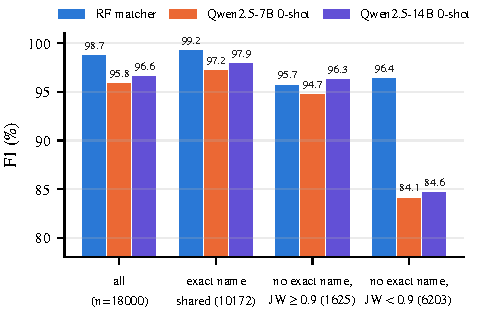
\includegraphics[width=\textwidth]{fig_strata.pdf}
\end{column}
\begin{column}{0.56\textwidth}
\small
\begin{itemize}
\item On the 7{,}828 test pairs with no exact shared name the forest keeps 96.1 F1 while the LLMs drop to 88 to 89. Deferring 10\% of this hard subset to a human lifts it to 99.5.
\item Trained on persons only and tested on organisations the forest gets 90.0, the other direction 97.8, and same-script to cross-script 97.1. The features transfer, but type-specific training matters.
\item Five cluster-size count features inflate F1 to 99.0 by leaking how often an entity appears in the data. They are dropped everywhere. Names alone give 97.0, attributes without names 97.4, both together 98.7.
\item 53\% of test pairs share no entity with training and the forest scores 99.1 F1 on them, so it is not memorising entities.
\end{itemize}
\end{column}
\end{columns}
\end{frame}

% ============================================================
\section{Conclusions}

\begin{frame}{Conclusions}
\begin{itemize}
\item A supervised classical matcher with 29 features reaches \hi{98.7 F1} on OpenSanctions Pairs, above zero-shot 7B and 14B LLMs and far above the published production scorer, with a few hundred labels.
\item Treating analyst review as a reject option, the calibrated confidence gate removes \hi{71\% of the remaining errors by reviewing 5\%} of pairs. Learned gates add nothing, a reviewer with 10\% error still helps, and the same rule adapts to asymmetric costs.
\item An LLM is a poor expert here. From 7B zero-shot up to a 32B model with reasoning it gains at most 0.25 F1, whether it is deferred to or combined with the matcher, because its error rate on the deferred pairs stays near the matcher's own and the 0.5\% hard core of attribute-poor same-name pairs stays hard.
\item Two artefacts of the raw benchmark, relational stubs and cluster-size counts, inflate supervised scores and have to be removed.
\item Limitations. The LLMs are open models up to 32B, the human is assumed to beat 24\% error on the deferred pairs, and the sample's class ratio is not the deployment ratio. Natural next steps are a frontier model on the deferred pairs and deployment-ratio evaluation.
\end{itemize}
\end{frame}

% ============================================================
\appendix
\begin{frame}{Backup. Gate quality and calibration}
\begin{columns}[T]
\begin{column}{0.5\textwidth}
\footnotesize AUC of each gate score on the test split\\[1mm]
{\scriptsize\begin{tabular}{@{}lcc@{}}
\toprule
gate score & vs matcher error & vs LLM gain\\
\midrule
confidence $\min(p,1-p)$ & \textbf{0.945} & \textbf{0.956}\\
GBT error gate & 0.932 & \\
LR error gate & 0.924 & \\
GBT gain gate & & 0.883\\
LR gain gate & & 0.926\\
\bottomrule
\end{tabular}}
\end{column}
\begin{column}{0.48\textwidth}
\small
\begin{itemize}
\item Isotonic calibration is fitted on the 6k validation pairs. The Brier score moves from 0.0140 to 0.0137 and the reliability curve lies on the diagonal.
\item The learned gates see the 29 features, the raw and calibrated probabilities, and are trained on 12k training pairs with LLM answers, disjoint from calibration and test data.
\item On the pairs deferred at a 10\% budget, 84\% have a missing date on one side (40\% elsewhere), 55\% are organisation pairs (33\%), and the matcher error rate is 14.4\% against 0.3\% on the kept pairs.
\end{itemize}
\end{column}
\end{columns}
\end{frame}

\end{document}
